\documentclass{my_article_class}

\begin{document}
%Kopfzeile
\ihead{WS 22/23}
 \chead{Statistik I - Tutorium}
 \ohead{}


\begin{titlepage}

\title{Statistik 1 Tutorium}
%\subtitle{\Large{\textit{Tutorium}}}
\author{}
\date{WS22/23}

\maketitle
\thispagestyle{empty}

\end{titlepage}


\newpage
\tableofcontents
\thispagestyle{empty}


\newpage
\setcounter{page}{1}


\section{Vorlesung}
\subsection{Was ist Statistik}

  \begin{tabular}{| c | c | c | c |}
    \hline
      \thead{Deskriptiv} & \thead{Inferenz} & \thead{amtliche Statistik} & \thead{Explorative Statistik} \\
    \hline
      \makecell{Merkmale, Zusammenhänge \\Grafische Darstellung \\Lage und Streumaße} &
      \makecell{GG  $\leftrightarrow$ Stichprobe\\ Stichprobenfehler(sample error)}   &
      \makecell{von Institutionen \\in Auftrag gegeben} &
      \makecell{Zusammenhänge in \\Daten finden, "Big Data",\\ etabliert in Wirtschaft} \\
    \hline
  \end{tabular}


\subsection{Grundgesamtheit und Stichprobe}
Grundgesamtheit: Menge der Objekte für die die Aussage der Untersuchung gelten soll\\
Stichprobe: regelgeleitete Auswahl einer Teilmenge von Elementen aus der Grundgesamtheit\\
Stichprobenfehler/Sampling Error: Merkmalsausprägung ist in GG und in Stichprobe unterschiedlich\\
Kleer hatte noch sampling:

Flick Stichproben Kapitel 4



\subsection{Variablen}
\subsubsection{Wiederholung Empirie 1 Hussy-Schreier-Echterhoff:}

\underline{1. Beschreiben:} Variable B hängt mit Variabale A zusammen\hspace{1cm}A \textemdash{} B\\\\
\underline{2. Erklären:}~~~~~~~~ Variable B ist abhängig von Variable A\hspace{2cm}A\textrightarrow B\\
Zusammenhang:\\
positiver Zusammenhang: A$\uparrow$ B$\uparrow$\\
negativer Zusammenhang: A$\uparrow$ B$\downarrow$ oder A$\downarrow$ B$\uparrow$\\ Kein Zusammenhang\\
\\ Kausalrelation:\\
A$\longrightarrow$B\\
A$\longleftarrow$B\\
A$\longleftrightarrow$B\\
\\Beide Zusammen:\\
A$\uparrow$ $\longrightarrow$ B$\downarrow$\\\\
\underline{3. erste und zweite Ordnung}\\
1. Ordnung: A $\longrightarrow$ B\\
2. Ordnung: A \textrightarrow x \textrightarrow B\\
x ist intervenierende Variable

\subsection{Skalenniveaus und diskret/stetig}


\begin{adjustbox}{valign=t}
\begin{forest}
 [Kategorial[Nominal[ungeordnet\\(Haarfarbe)]][Ordinal[geordnet\\(Schulnoten)]]]
\end{forest}
\end{adjustbox}\qquad
\begin{adjustbox}{valign=t}
\begin{forest}
 [Metrisch  [Intervall[Konstante\\Abstände\\(Temperatur \celsius)]][Ratio[natürlicher\\Nullpunkt\\(Kelvin)]]]
\end{forest}
\end{adjustbox}
\vspace{0.5cm}\\
Pseudometrisch: Ordinal wird oft als Intervall behandelt, wenn genug Ausprägungen vorhanden sind\\
Welches Skalenniveau haben folgende Variablen?
\begin{enumerate}
\item Selbstvertrauen: hoch, mittel, niedrig \solution{Ordinal}
\item Jahreszahl (z.B. 1982)                 \solution{Intervall}
\item Alter                                  \solution{Ratio}
\item Geschlecht                             \solution{Nominal}
\item Anzahl erreichter Creditpoints         \solution{Ratio, 1CP=30h\textrightarrow so als ob nach <Stunden> gefragt wird}
\item Einkommen                              \solution{Ratio}

\end{enumerate}
\vspace{0.5cm}
diskret: Endlich Viele Werte können angenommen werden~1--------------------------2
\\stetig:~~~~Annahme eines beliebigen Wertes in Intervall~~~~~~~~~~~1--1.1--1.127587-------2
\vspace{0.5cm}
\\Sind die folgenden Variablen diskret oder stetig?
\begin{enumerate}
\item Gewicht                                \solution{Stetig}
\item Jahreszahl (z.B. 1982)                 \solution{Diskret}
\item Alter                                  \solution{Stetig}
\item Exakte Zeit eines 100m Läufers         \solution{Stetig}
\item Geschlecht                             \solution{Diskret}
\item Einkommen                              \solution{Stetig}
\end{enumerate}
\vspace{0.5cm}
\underline{Kleer hatte noch:}
\\dichotom: 2 Ausprägungen
\\polytom: Mehr als 2 Ausprägungen
\\
\\Makro: aggregierte Daten
\\Mikro: Individualdaten
\\
\\latent: nicht direkt beobachtbar
\\manifest: messbar
\\

\section{Vorlesung}

Ziel der Vorlesung: Studierende können univariate Analysen machen\\


\subsection{Datenmatrix}
\begin{itemize}
 \item auch \textit{Urliste} genannt
 \item Spalten $\rightarrow$ Variablen
 \item Zeilen  $\rightarrow$ Fälle
 \item Jeder Fall bekommt eine ID zugewiesen
\end{itemize}
==> Aufgabe 1 Serdar
\subsection{Häufigkeiten}
\textbf{f}requenz und \textbf{H}äufigkeit
\begin{itemize}
 \item [1.] \textbf{Absolute Häufigkeit:}~~ $fx_k = Hx_k$
 \item [2.] \textbf{Relative Häufigkeit:}~~ $\frac{fx_k}{n} = hx_k$
 \item [3.] \textbf{prozentuale Häufigkeit:}~~ $hx_k \cdot 100$
\end{itemize}

\subsection{kumulierte Häufigkeit}
politisches Interesse Allbus:\\
\begin{tabular}[h]{r|c|c|c|l}
        Kategorie   & $Hx_k$    &  $hx_k$   &  $hx_k \cdot 100$ & kumulierte prozentuale Häufigkeit  \\
  \hline
	sehr stark  & 425       & 0,122    & 12,2 & 12,2\\
        stark       & 877       & 0,251    & 25,1 & 37,3\\
        mittel      & 1437      & 0,412    & 41,2 & 78,5\\
        wenig       & 564       & 0,162    & 16,2 & 94,7\\
überhaupt nicht     & 186       & 0,053    & 5,3  & 100\\
  \hline
	Gesamt & 3490 & 1,000 & 100 & {}\\
\end{tabular}
\begin{enumerate}
\item Wie viele Menschen sind mindestens stark politisch interessiert? \solution{37,3\%}
\item Wie hoch ist der prozentuale Anteil der Personen, die weniger als <mittel> interessiert sind? \solution{$100\% - 37,3\% = 62,7\%$}
\item Wie hoch ist der prozentuale Anteil der Personen, <stark, mittel, wenig> angekreuzt haben? \solution{$94,7\% - 12,2\% = 82,5\% $}
\item Welche Häufigkeitsdarstellung zeigt am besten wie viele Individuen der Stichprobe vor dem 55. Lebensjahr in Rente gegangen sind? \solution{kumulative Häufigkeitsverteilung}
\end{enumerate}

\subsection{Darstellungsarten}
\begin{tabular}{r|l|l}
      {} & Variablenskala & zu beachten \\
\hline
Piechart & nominal        & nur wenig Kategorien\\
Säulendiagramm & nominal, ordinal & Reihenfolge auf X-Achse\\
Histogramm & intervall, ratio & hat Zweck Fläche darzustellen \textrightarrow Polygonzug/Dichteverteilung mit angeben  \\
\end{tabular}
\begin{figure}[h]
 \centering
 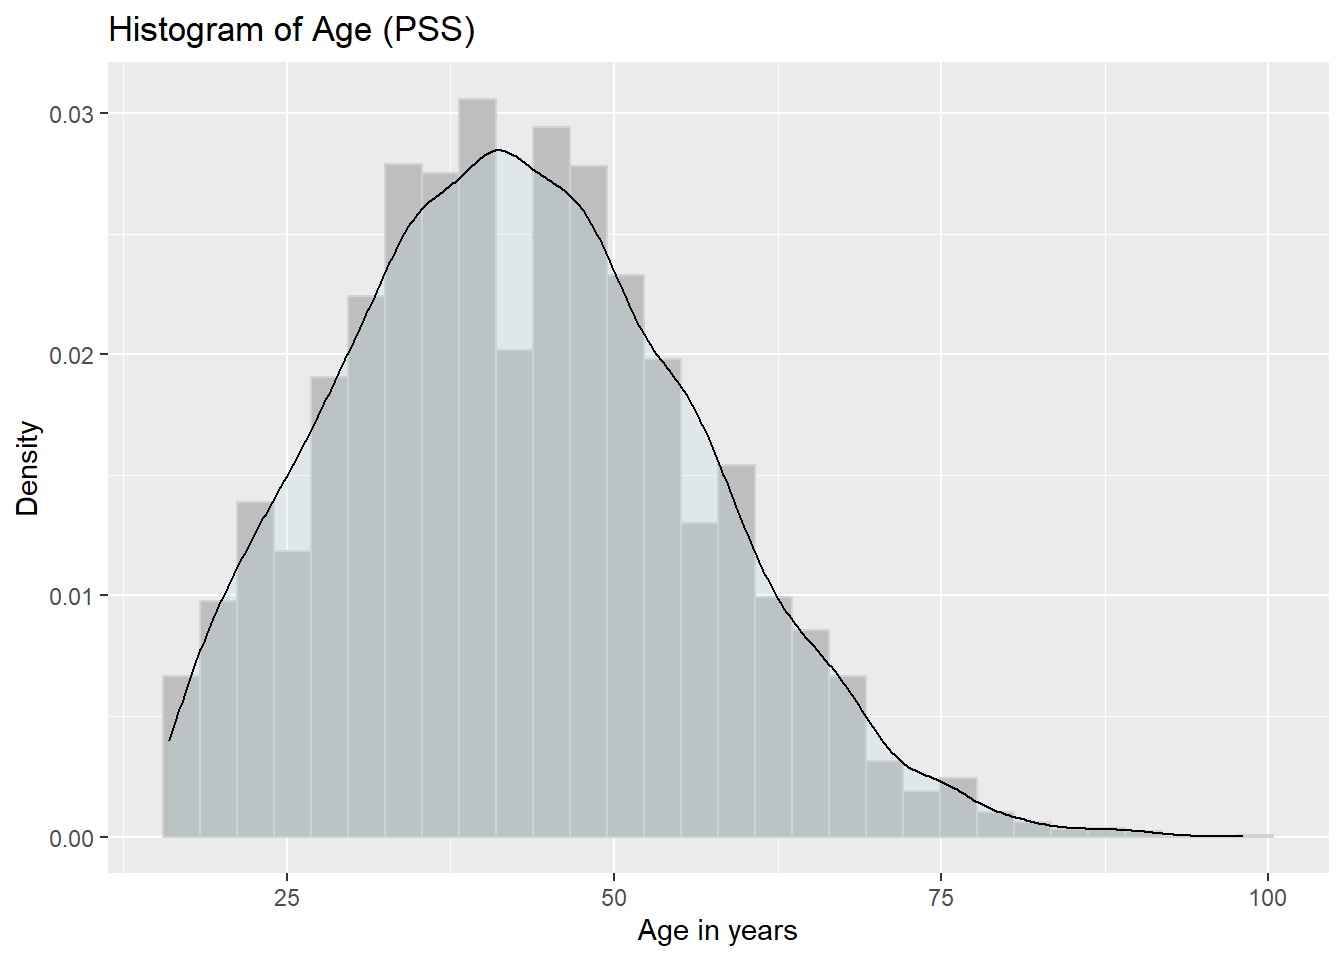
\includegraphics[scale=0.6]{./img/hist-density-1.png}
 \caption{Histogramm mit Dichteverteilung}
\end{figure}

\subsection{Verteilungsformen}
Symetrisch\\
Bimodal\\
linkssteil,rechtsschief\\
rechtssteil,linksschief\\
\\
\subsection{Summenzeichen}
$\sum_{i=m}^{n}a_i~~~=~~~a_{m} + a_{m+1} + a_{m+2} + a_{m+3} + \dots + a_{n}$
\\
Für alle Aufgaben gilt folgende Tabelle:
\begin{tabular}{c|ccccc}
    $\textrm{a}_\textrm{i}$ & $\textrm{a}_\textrm{1}$ & $\textrm{a}_\textrm{2}$ & $\textrm{a}_\textrm{3}$ & $\textrm{a}_\textrm{4}$ & $\textrm{a}_\textrm{5}$ \\ \hline
    x & 2 & 1 & 5 & 3 & 3
\end{tabular}

\begin{align*}
  A &= \sum_{i=1}^{n}x_{i}  &
  B &= \sum_{i=2}^{4}x_{i} &
  C &= \sum{x_{i}} &
  D &= \sum{x_{i}}^2 &
  E &= (\sum_{i=1}^{n}{x_{i}})^2 &\\\\
  F &= (\sum_{i=1}^{n}{x_{i}})-1 &
  G &= \sum_{i=1}^{n}(x_{i}-1) &
  H &= \sum_{i=1}^{n}(x_{i}-1)^2 &
  I &= (\sum_{i=1}^{n}(x_{i}-1))^2 &
  J &= \frac{\sum_{i=1}^{n}(x_{i}-1)}{n} &\\\\
  K &= \frac{\sum_{i=1}^{n}(x_{i}-2)^2}{n} &
  L &=  &
  M &=  &
  N &=  &
  O &=  &\\
\end{align*}
Lösungen:
\begin{tabular}{c|c|c|c|c|c|c|c|c|c|c|c|c|c|c}
    A  & B & C  & D  & E        & F  & G & H  & I        & J                 & K  & L  & M  & N  & O\\
    14 & 9 & 14 & 48 & $14^{2}$ & 13 & 9 & 25 & 81       & $\frac{9}{5}=1,8$ & $\frac{12}{5}$ & {} & {} & {} & {}
\end{tabular}

\section{Vorlesung}


\subsection{Lagemaße/Maße der zentralen Tendenz}
\begin{tabular}{r|l|l}
     Modus                  & Wert kommt am häufigsten vor       & ratio, intervall, ordinal, nominal\\
     Median                 & Teilt Menge in 2 gleichgroße Teile & ratio, intervall, ordinal \\
     arithmetisches Mittel  & Durchschnitt                       & ratio, intervall
\end{tabular}


\subsubsection{Median}
\begin{tabular}{r|c|l}
     n - ungerade &$\widetilde{x}~=~x_{\frac{n+1}{2}}$&  \\
     {}&{}&{}\\
     n - gerade   &$\widetilde{x}~=~\frac{x_{\frac{n}{2}}+x_{\frac{n}{2}+1}}{2}$&
\end{tabular}\\\\
\\ungerade:
\begin{tabular}{cc|c|cc}
     $x_{1}$&$x_{2}$&$x_{3}$&$x_{4}$&$x_{5}$  \\
     3&5&6&8&12
\end{tabular}\\
mittlerer Wert = 6\\
\\
gerade :
\begin{tabular}{cc|cc|cc}
     $x_{1}$&$x_{2}$&$x_{3}$&$x_{4}$&$x_{5}$&$x_{6}$  \\
     3&5&6&8&12&13
\end{tabular}\\
Durchschnitt der mittleren beiden Werte = 7


\subsubsection{arithmetische Mittel}
\begin{equation*}
    \overline{x}=\frac{\sum_{i=1}^{n}x_{i}}{n}~~~~~\leftarrow \textrm{Datenmatrix (``normale'' Formel)}
\end{equation*}
  \vspace{0.5cm}
\begin{equation*}
     \overline{x}=\frac{\sum_{k=1}^{m}(x_{k}\cdot f_{{x}_{k}})}{n}~~~~~\leftarrow \textrm{Häufigkeitstabelle (``spezial'' Formel)}
\end{equation*}


\underline{Erläuterung der Gleichungen:}\\
Um die mittlere Antwort, einen ``Durchschnitt'', zu berechnen werden zuerst alle Antworten die gegeben wurden aufsummiert und im zweiten Schritt durch die Anzahl der Antworten (n) geteilt.\\

In der Datenmatrix/Urliste sind alle Antworten als $x_i$'s direkt ablesbar. Diese können einfach aufsummiert werden. Die Anzahl aller Antworten (n) kann an der ID des letzten Falls abgelesen werden (sofern keine Fälle dazwischen herausgefiltert wurden).\\

In der Häufigkeitstabelle kann man die einzelnen Antworten nicht so direkt ablesen wie in der Datenmatrix. Jedoch wissen wir, dass bspw. 400 Personen Antwortausprägung 1 gegeben haben, 600 Antwortausprägung 2 usw.. Antwort 1 kommt also 500 \textit{mal} in der Datenmatrix vor, Antwort 2 600 \textit{mal} usw.. Wir rechnen also die jeweilige Antwort \textit{MAL} die Anzahl wie oft diese Antwort angegeben wurde. Die Anzahl aller Antworten (n) wird ermittelt indem die Häufigkeiten der einzelnen Antwortausprägungen addiert werden.

\subsection{Dispersionsmaße/Lagemaße und Verteilungsformen}
\textbf{Verteilungsübersicht:}\\
\begin{tabular}{|c|c|}
\hline
    Modus < Median < arithmet.Mittel & linkssteil/rechtsschief
\\ \hline
    arithmet.Mittel < Median < Modus & rechtssteil/linksschief
\\ \hline
    2 Modi, Median = arithmet.Mittel, Modus weicht stark ab & bimodal
\\ \hline
    arithmet.Mittel,Modalwert und Median fast gleich & symetrisch\\
  \hline
\end{tabular}


\subsubsection{Übung}
\begin{enumerate}
\item Berechne den Median für folgende Werte: 5,2,4,4,3,5,8 \solution{4}
\item Was ist der Modus der folgenden Werte? 3,3,4,4,4,5,5,5,5,2,2,1,1,0 \solution{5}
\item Um welche Art der Verteilung besitzt folgende Werte: arithmetisches Mittel =  24, Modus = 32, Median = 27 \solution{rechtssteil/linksschief}
\end{enumerate}

\section{Vorlesung}

\subsection{Variationsweite/Spannweite/Range}
\begin{equation*}
    V = x_{max} - x_{min}
\end{equation*}
Beispiel: höchster Wert: 10, niedrigster Wert 7 \\\textrightarrow 10 - 7 = 3 = IQR\\
Nachteil: Starke Abweichungen einzelner Werte können zu Fehlinterpretationen führen.

\subsection{Interquartilabstand/IQR}
\begin{equation*}
    IQR = Q_{0.75} - Q_{0.25}
\end{equation*}

\subsection{Varianz}
\textrightarrow durchschnittliche Abweichung, Voraussetuzung: Pseudometrisches Skalenniveau
\begin{align*}
    \sigma^{2}& = \frac{\sum_{i=1}^{n}(x_{i}-\overline{x})^2}{n}~~~\longleftarrow \textrm{Varianz für Grundgesamtheit}\\
    \textrm{s}^{2}& = \frac{\sum_{i=1}^{n}(x_{i}-\overline{x})^2}{n-1}~~~\longleftarrow \textrm{Varianz für Stichprobe}
\end{align*}

\subsection{Standardabweichung}
\begin{align*}
    \sigma^{2}& = \frac{\sum_{i=1}^{n}(x_{i}-\overline{x})^2}{n}~~~\longleftarrow \textrm{Varianz}\\
    \sqrt{\sigma^{2}}& = \sigma~~~\longleftarrow \textrm{Standartabweichung}
\end{align*}
\textbf{\underline{Beispiel:}}\hfill(von \href{https://de.statista.com/statistik/lexikon/definition/126/standardabweichung/#:~:text=Definition%20Standardabweichung,Auspr%C3%A4gungen%20eines%20Merkmals%20vom%20Durchschnitt.}{Statista})\\
Gefragt wurden 1.000 Personen, wie hoch ihre monatliche Handyrechnung ist. Der Mittelwert liegt bei 40 Euro und die Standardabweichung bei 27. Das heißt, dass die durchschnittliche Entfernung aller Antworten zum Mittelwert 27 Euro beträgt.\\
Man würde wiefolgt schreiben:
\begin{align*}
  \overline{x}&= 40\textrm{\EUR}\\
  \sigma&= 27\textrm{\EUR}\\
  \overline{x}&= 40\pm27\textrm{\EUR}
\end{align*}

\subsection{Übung}
Der IQR sind die mittleren 50\% der Verteilung.
\begin{figure}[h]
 \centering
 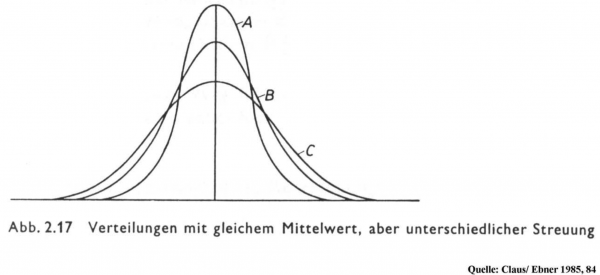
\includegraphics[scale=0.6]{./img/IQR_1.png}
 \caption{IQR}
\end{figure}
\vspace{0.5cm}
\begin{enumerate}
\item Ordne die IQRs der Verteilungen nach Größe. \solution{$IQR_{A} < IQR_{B} < IQR_{C}$}
\item Wie lautet die Standardabweichung und der Mittelwert für die folgenden Werte 44,67,102,42,52,42 \solution{circa 21,45}
\item Wie lautet die Standardabweichung für folgende Zahlen:\\
1,2,3,4,5 \solution{Varianz: 2; Standardabweichung: $\sqrt{2}$ }
\end{enumerate}


\section{Vorlesung}


\subsection{Quantile}
Quartile sind eine Art Quantile. Sie teilen die Anzahl der Werte in gleich große Teile. Quartile teilen mithilfe von 3 Wertegrenzen die Anzahl der Werte in 4 gleichgroße Teile je 25\%.



\subsection{Boxplots}
  \small{\textbf{\textrightarrow (pseudo-) metrisch}}
\vspace{1cm}
  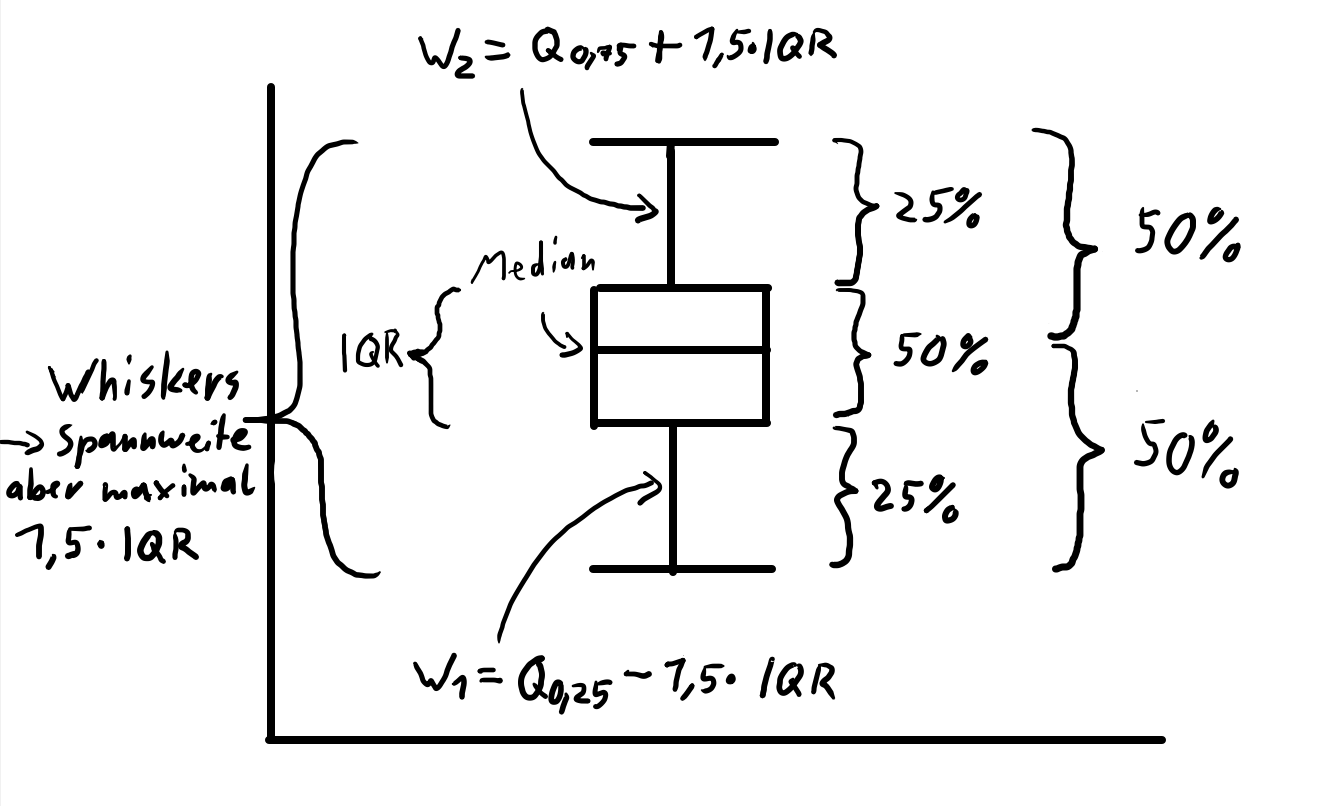
\includegraphics[scale=0.25]{./img/Boxplot.png}

\subsubsection{Ausreißer und Extremwert}
\begin{tabular}{l|l}
  Ausreißer & = \textcolor{red}{1,5~$\cdot$~IQR}~~~über 3. Quartil/ unter 1. Quartil\\
  Extremwert& =\textcolor{red}{~~~~3~$\cdot$~IQR}~~~über 3. Quartil/ unter 1. Quartil
\end{tabular}



\subsection{Variantionskoeffizient V}
  Mit dem Variantionskoeffizienten kann man \textbf{Streuungen} verschiedener Verteilungen vergleichen.
\begin{align*}
  \textrm{V} = \frac{\sigma}{\overline{x}} = \frac{\textrm{Standardabweichung}}{\textrm{arithm. Mittel}} && ;\overline{x}\neq 0
\end{align*}

\subsection{Z-Transformation oder Z-Wert}
  Mit dem Z-Wert kann man \textbf{Werte} verschiedener Verteilungen vergleichen. (In Statistik 2 wird die Z-Transformation im Zusammenhang mit der Standardnormalverteilung sehr wichtig.\\(\href{https://youtu.be/2tuBREK_mgE?t=163}{Ein interessantes Youtubevideo, es nimmt allerdings schon einige Zusammenhänge vorweg, die später nocheinmal richtig in Statistik 2 vorkommen}))


\begin{align*}
 \textrm{z} &= \frac{x_{\textrm{i}} - \overline{x}}{\sigma}
\end{align*}
- Mittelwert aller Z-Werte = 0\\
- Varianz    aller Z-Werte = 1

\begin{comment}
\subsection{Übung}
\begin{enumerate}
\end{enumerate}
\end{comment}

%Aufgabe zu variantionskoeffizient einfügen

\newpage
\section{Vorlesung}

\subsection{Kreuztabelle/ Kontingenztafel}

  \begin{itemize}
    \item für nominale/ordinale Variablen
    \item Konvention: Zeile-Abhängig/Spalte-unabhängig
  \end{itemize}
\vspace{1cm}
Beispieltabelle(fiktional): \\
 \begin{itemize}
   \item [x] =~~~Studierende besuchen das Tutorium
   \item [y] =~~~Studierende bestehen die Statistikklausur
   \item [] Nichtantritt = nicht bestanden
 \end{itemize}

 \begin{tabular}{p{2cm}|p{2cm}|p{2cm}|p{2cm}}
    {}              & Tutorium besucht & Tutorium nicht besucht & \textit{Gesamt}
\\\hline
    bestanden       & 9                & 59                     & 68
\\\hline
    nicht bestanden & 2                & 14                     & 16
\\\hline
    \textit{Gesamt} & 11               & 73                     & 84
 \end{tabular}

 \subsection{Übung}
  \begin{enumerate}
    \item Wie hoch ist der relative Anteil aller eingeschriebenen Studierenden die das Tutorium nicht besucht und die Klausur nicht bestanden haben?
      \solution{$\frac{14}{84} = 16,6\%$}

    \item Wie hoch ist der relative Anteil aller eingeschriebenen Studierenden die die Klausur bestanden haben?
      \solution{$\frac{68}{84} = 80,9\%$}

    \item Wie hoch ist der relative Anteil der Tutoriumsbesucher, die die Klausur bestanden haben?
      \solution{$\frac{9}{11} = 81,8\%$}

    \item Wie viel Prozent aller bestehenden Studierenden haben das Tutorium besucht?
      \solution{$\frac{9}{68} = 13,2\%$}
 \end{enumerate}
\vspace{1cm}
Ergänze folgende Kreuztabelle (\href{https://www.destatis.de/DE/Themen/Gesellschaft-Umwelt/Gesundheit/Gesundheitszustand-Relevantes-Verhalten/Tabellen/liste-rauchverhalten.html#119170}{Statistisches Bundesamt 2021}):\\
\begin{tabular}{p{2cm}|p{2cm}|p{2cm}|p{2cm}}
   Geschlecht x Rauchen & Raucher            & Nichtraucher           & \textit{Gesamt}
\\\hline
   männlich             & 5059               & A                      & 22 684
\\\hline
   weiblich             & B                  & C                      & 23 547
\\\hline
   \textit{Gesamt}      & 8 738              & D                      & 46 231
\end{tabular}

\begin{enumerate}
  \item A \solution{22684 - 5059 = 17625}
  \item B \solution{8738  - 5059 = 3679 }
  \item C \solution{23547 - 3679 = 19868}
  \item D \solution{17625 + 19868= 37493}
\end{enumerate}

\section{Vorlesung (Zusammenhang zwischen nominal und ordinalskalierten Variablen)}

\subsection{Kreuztabellen}
Es gibt 2 Arten von Kreuztabellen:
\begin{itemize}
  \item [1.] Kontingenztabelle - enthält beobachtete Werte
  \item [2.] Indifferenztabelle - enthält erwartete Werte
\end{itemize}

\subsection{Erwartete Häufigkeit}
\begin{align*}
  \textrm{f}_\textrm{e(ij)} = \frac{Zeilensumme \cdot Spaltensumme}{n}
\end{align*}
\underline{\textbf{Erklärung:}}\\
Die Gleichung kann leicht umgestellt werden in: $\textrm{f}_\textrm{e(ij)} = Zeilensumme \cdot \frac{Spaltensumme}{n}
$. Nun wird deutlich, dass ''Spaltensumme durch n'' ein Prozentsatz ist (äquivalent ergibt sich $Spaltensumme \cdot \frac{Zeilensumme}{n}$, was im Grunde dasselbe ist).

Dieser Zeilensummenprozentsatz wird nun durch das Malrechnen auf alle Fälle der jeweiligen Spalte der Zelle angewendet. So entsteht der erwartete Wert.\\
\\\\
\underline{Residuen}: Differenz beobachteter und erwarteter Werte\\ je höher dieser Unterschied ist, desto eher kann man einen Zusammenhang vermuten


\subsection{Chi-Quadrat}
\begin{align*}
\chi^{2}~~=~~\sum_{i=1}^{k} \sum_{j=1}^{m} \frac{(\textrm{f}_{\textrm{b}_{\textrm{ij}}} - \textrm{f}_{\textrm{e}_{\textrm{ij}}})^2}
{\textrm{f}_{\textrm{e}_{\textrm{ij}}}}
\end{align*}
\underline{\textbf{Erklärung:}}\\
Für jede Zelle werden die Abstände von beobachtetem und erwartetem Wert(Residuen) berechnet($\textrm{f}_{\textrm{b}_{\textrm{ij}}} - \textrm{f}_{\textrm{e}_{\textrm{ij}}}$). Da wir nur an den positiven Abständen interessiert sind (wie schon bei der Varianz) wird das Residuum der Zelle quadriert. Nun wird durch den erwarteten Wert geteilt,, weil wir von keinem Zusammenhang, also den erwarteten Werten ausgehen. Alles was wir bisher gerechnet haben wird für alle Zellen gerechnet und zusammengezählt. Das wird in der Gleichung damit erreicht, dass alle Spalten aufsummiert werden ($\sum_{j=1}^{m}$) und diese Ergebnisse für alle Zeilen summiert werden ($\sum_{i=1}^{k}$).
\\
\begin{enumerate}
  \item $0 < \chi^2 < \infty (nicht standardisiert)$
  \item Je größer der Wert desto größer der Zusammenhang (0: kein Zusammenhang)
\end{enumerate}
\vspace{0.5cm}
\underline{\textbf{\size{20}{ABER!!!}~~~Abhängig von n und der Variablenzahl.}}


\subsection{Normierung Chi-Quadrat mit Phi, Cramers V, C}

\subsubsection{Phi}
$\phi$ korrigiert die Abhängigkeit von n. Es ist sinvoll in die Analyse mit einzubeziehen, wenn man den Zusammenhang unabhängig von der Gesamtfallzahl interpretieren möchte.
\begin{align*}
  \phi =  \sqrt{\frac{\chi^2}{n}}
\end{align*}
\begin{itemize}
  \item [-] $0 < \phi < 1$, wobei 0: kein Zusammenhang, 1: max. Zusammenhang
\end{itemize}

\subsubsection{Kontingenzkoeffizient C}
$C$ korrigiert die abhängigkeit von der Variablenanzahl. Es ist mega unwichtig, wird nur selten gelehrt. Der Grund dafür ist, dass der Versuch unabhängig von der Kategorienanzahl interpretieren zu können schief geht. Die Kategorienzahl muss wieder bei der Berechnung von $C_{max}$ mit einbezogen werden.
\begin{itemize}
  \item [-] $0 < C < C_{\textrm{max.}}$, wobei 0: kein Zusammenhang, $C_{max}$: max. Zusammenhang
\end{itemize}
\begin{align*}
  C &= \sqrt{\frac{\chi^2}{\chi^2 + n}}\\
  C_{\textrm{max}} &= \sqrt{\frac{R-1}{R}}~~~~~~~~~~~~~~~~\textrm{;R = Minimum Zeilen-/Spaltenanzahl}
\end{align*}
Beispiele für R:
\begin{itemize}
  \item [$2\times2:$] R = 2
  \item [$3\times4:$] R = 3
  \item [$4\times3:$] R = 3
\end{itemize}

\subsubsection{Cramer's V}
Cramer's V wird für den Vergleich von $\chi^2$ aus verschieden großen Kreuztabellen genutzt.
\begin{itemize}
  \item [-] 0 < Cramer's < 1
\end{itemize}
\begin{align*}
  \textrm{Cramer's V} = \sqrt{\frac{\chi^2}{\chi^2_{\textrm{max}}}} = \sqrt{\frac{\chi^2}{n\cdot(R - 1)}} = \sqrt{\frac{\chi^2}{n\cdot(\textrm{min}(k,m)-1)}}
\end{align*}

\subsection{Interpretation Phi und Cramer's V}
\begin{tabular}{l|l}
  Cramer's V bzw. Phi & Interpretation \\
\hline
  $\leq 0,05$     & kein Zusammenhang \\
  > 0,05 bis 0,10 & sehr schwacher Zusammenhang \\
  > 0,10 bis 0,20 & schwacher Zusammenhang \\
  > 0,20 bis 0,40 & mittelstarker Zusammenhang \\
  > 0,40 bis 0,60 & starker Zusammenhang \\
  > 0,60          & sehr starker Zusammenhang
\end{tabular}
\newpage

\subsection{Übung}
\begin{figure}[h!]\centering
\begin{tabular}{p{2cm}|p{2cm}|p{2cm}|p{2cm}}
   Geschlecht x Rauchen & Raucher            & Nichtraucher           & \textit{Gesamt}
\\\hline
   männlich             & 5 059              & 17 625                 & 22 684
\\\hline
   weiblich             & 3 679              & 19 868                 & 23 547
\\\hline
   \textit{Gesamt}      & 8 738              & 37 493                 & 46 231
\end{tabular}
\caption{Statistisches Bundesamt 2021}
\small{\url{https://www.destatis.de/DE/Themen/Gesellschaft-Umwelt/Gesundheit/Gesundheitszustand-Relevantes-Verhalten/Tabellen/liste-rauchverhalten.html#119170}}
\label{7_raucher}
\end{figure}

\begin{enumerate}
  \item Berechne und interpretiere $\chi^2$ für die Tabelle. \solution{336.138 Im Verhältnis zur Größe der Fallzahl ist der Wert ziemlich gering.\textrightarrow kein Zusammenhang}
  \item Berechne und interpretiere $\phi$ \solution{$\phi$ = 0,0125~~~~~Da 0<$\phi$<1 \textrightarrow kein Zusammenhang}
  \item Berechne C max \solution{$C = 215; C_{max} = 0.7$ Meine Werte sind sicherlich falsch. Diese kontrollieren wir gerne zusammen im Tutorium\textrightarrow kein Zusammenhang}
  \item Berechne und interpretiere Camer's V \solution{V = 0.085 Cramers V ist sehr gering \textrightarrow kein Zusammenhang}
\end{enumerate}

\section{Vorlesung}

\subsection{Spearman's Rho/Rangkorrelationskoeffizient}
Spearman's $\rho$ (Rangkorrelationskoeffizient) findet Anwendung, wenn beide Variablen ordinal, metrisch oder ordinal und metrisch skaliert sind.
\begin{align*}
  \rho &= 1 - \frac{6 \cdot \sum^{n}_{i=1}{d^2_i}}{n \cdot (n^2-1)}\\
  d_i  &= R(x_i) - R(y_i)~~~\textrm{(Differenz der Rangplätze)}\\
  &-1 < \rho < 1
\end{align*}
\textbf{\underline{Erklärung:}} \\
\underline{Ursprung der Formel:} Die Formel ergibt sich (Achtung, vorgriff auf nächste Vorlesung) aus einem Spezialfall von Pearson's r. Es muss lediglich statt den wahren Werten Ränge eingesetzt werden um die Formel zu erhalten. \\
\underline{\textbf{Herleitung:}}\hspace{15cm}\href{https://stats.stackexchange.com/questions/89121/prove-the-equivalence-of-the-following-two-formulas-for-spearman-correlation}{Quelle}
\begin{align*}
  \rho &= \frac{\sum_i(x_i-\bar{x})(y_i-\bar{y})}{\sqrt{\sum_i (x_i-\bar{x})^2 \sum_i(y_i-\bar{y})^2}} = \frac{\sum_i(x_i-\bar{x})(y_i-\bar{y})}{\sum_i (x_i-\bar{x})^2}~~~~~\textrm{weil es keine Gleichstände gibt und} x,y\in\{1,2,...,n\}\\
  \textrm{Nenner:}&\\
  &\sum_i (x_i-\bar{x})^2 ~~=~~ \sum_i x_i^2 - n\bar{x}^2 \\
&= \frac{n(n + 1)(2n + 1)}{6} - n(\frac{(n + 1)}{2})^2
~~=~~ n(n + 1)(\frac{(2n + 1)}{6} - \frac{(n + 1)}{4})\\
&= n(n + 1)(\frac{(8n + 4-6n-6)}{24})
~~=~~ n(n + 1)(\frac{(n -1)}{12})\\
&= \frac{n(n^2 - 1)}{12}\\
\textrm{Zähler:}&\\
&\sum_i(x_i-\bar{x})(y_i-\bar{y}) ~~=~~ \sum_i x_i(y_i-\bar{y})-\sum_i\bar{x}(y_i-\bar{y})  ~~=~~ \sum_i x_i y_i-\bar{y}\sum_i x_i-\bar{x}\sum_iy_i+n\bar{x}\bar{y} \\
&=\sum_i x_i y_i-n\bar{x}\bar{y} ~~=~~ \sum_i x_i y_i-n(\frac{n+1}{2})^2 ~~=~~ \sum_i  x_i y_i- \frac{n(n+1)}{12}3(n +1) \\
&= \frac{n(n+1)}{12}.(-3(n +1))+\sum_i  x_i y_i ~~=~~ \frac{n(n+1)}{12}.[(n-1) - (4n+2)] + \sum_i  x_i y_i \\
&= \frac{n(n+1)(n-1)}{12} - n(n+1)(2n+1)/6 + \sum_i  x_i y_i ~~=~~ \frac{n(n+1)(n-1)}{12} -\sum_i x_i^2+ \sum_i  x_i y_i \\
&= \frac{n(n+1)(n-1)}{12} -\sum_i (x_i^2+ y_i^2)/2+ \sum_i  x_i y_i  ~~=~~ \frac{n(n+1)(n-1)}{12} - \sum_i (x_i^2 - 2x_i y_i + y_i^2) /2\\
&= \frac{n(n+1)(n-1)}{12} - \sum_i(x_i - y_i)^2/2 ~~=~~ \frac{n(n^2-1)}{12} - \sum d_i^2/2\\
\textrm{Beide Zusammenfügen:}&\\
&= \frac{n(n+1)(n-1)/12 - \sum d_i^2/2}{n(n^2 - 1)/12} ~~=~~ {\frac {n(n^2 - 1)/12 -\sum d_i^2/2}{n(n^2 - 1)/12}} ~~=~~ 1- {\frac {6 \sum d_i^2}{n(n^2 - 1)}}
\end{align*}
Ich habe die Herleitung hier eingefügt um zu zeigen, dass an diesem Punkt der Vorlesung Schulmathematik vielleicht noch mit Mathe Leistungskurs zum Herleiten ausreicht, allerdings an seine Grenzen stößt. Formeln wie diese können von Nichtmathematikern allerdings durch Kontext und Anwendung versucht werden zu verstehen.\\
\\
\underline{\textbf{Anwendung und Beispiel(fiktiv):}}
Wir gehen von folgender Tabelle aus:\\
\begin{tabular}[h!]{l|cc}
ID & Anzahl Tutoriumsbesuche & Klausurnote \\\hline
1 & 0 & 8 \\
2 & 3 & 9 \\
3 & 0 & 6 \\
4 & 1 & 5 \\
5 & 12& 12\\
6 & 10& 13\\
\end{tabular}\\
Nun werden den Werte Ränge zugewiesen, also vom kleinsten Wert bis zum größten Wert durchnummeriert. Sollte ein Wert doppelt (Im Beispiel die 0) vorkommen, wird beiden der Durchschnitt des Ranges zugeordnet. 0 hat Rang 1, weil 0 zweimal vorkommt bilden wir den Durchschnitt der Ränge. Einer Null wird also Rang 1 zugeordnet, der anderen Rang 2 und der Durchschnitt ist 1,5. Die 1,5 wird beiden zugeordnet.\\
\begin{tabular}[h!]{l|cc}
ID & Ränge der Anzahl Tutoriumsbesuche & Ränge der Klausurnote \\\hline
1 & 1,5 & 3 \\
2 & 3   & 4 \\
3 & 1,5 & 2 \\
4 & 2   & 1 \\
5 & 5   & 5 \\
6 & 4   & 6 \\
\end{tabular}\\
Im Anschluss wird die Differenz der Ränge ($d_i$) berechnet:\\
\begin{tabular}[h!]{l|cc}
ID & Ränge der Anzahl Tutoriumsbesuche & Ränge der Klausurnote & $d_i$ \\\hline
1 & 1,5 & 3 & 1,5\\
2 & 3   & 4 & 1  \\
3 & 1,5 & 2 &0,5 \\
4 & 2   & 1 & 1  \\
5 & 5   & 5 & 0  \\
6 & 4   & 6 & 2  \\
\end{tabular}\\
\begin{align*}
\rho &= 1 - \frac{6 \cdot \sum^{n}_{i=1}{d^2_i}}{n \cdot (n^2-1)}~~~~~\textrm{Summe ausformulieren\textrightarrow Ränge einsetzen}\\
&= 1 - \frac{6 \cdot (1,5^2 + 1^2 + 0,5^2 + 1^2 + 0^2 + 2^2)}{n \cdot (n^2-1)}~~~~~\textrm{Ränge zusammenrechnen und n einsetzen}\\
&= 1 - \frac{6 \cdot (2,25 + 1 + 0,25 + 1 + 4)}{n \cdot (6^2-1)}~~~~~\textrm{weiter zusammenfassen}\\
&= 1 - \frac{6 \cdot 8,5}{6 \cdot (6^2-1)}~~~~~\textrm{weiter zusammenfassen}\\
&= 1 - \frac{51}{6 \cdot (36-1)}~~=~~1 - \frac{51}{6 \cdot 35}~~=~~1 - \frac{51}{210}~~=~~1 - 0,243 ~~=~~0,757
\end{align*}

%\input{./VL/VL_9}
%\input{./VL/VL_10}


%Übung zur Datendarstellung und Analyse ausdenken


\end{document}
